\documentclass[../TM3-UltraDoc.tex]{subfiles}
\begin{document}
	\section*{6) Weighted graph}
	\addcontentsline{toc}{section}{6) Weighted graph}
	% Your content here
	\textbf{Взвешенный граф (Weighted graph)} - граф в котором у кадого ребра есть вес (взвешенные ребра)\\
	\\
	Более формально - с каждым ребром есть ассоциированное численное значение - вес, представляемое в виде весовой функции.\\
	\textit{Не кидайтесь в меня тапками, я буквально перевел на русский то, что написано в читшите}\\
	\\
	Еще более формально - Взвешенный граф\\ 
	\(G = \langle V, E, w \rangle; \\ w: E \rightarrow Num\) \\
	\textit{это то что написано в читшите, мне лично понятнее вот так:}\\
	\(w: e \in E \rightarrow weight_e\)\\
	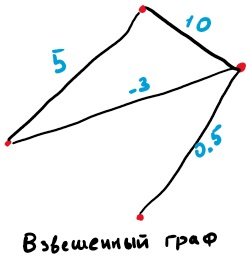
\includegraphics[width = 0.4\textwidth]{6.1}
\end{document}